%% IEEE TNNLS Paper Draft
%% Composed from ch1new.tex - ch5new.tex
%%
\documentclass[journal]{IEEEtran}

% *** PACKAGES ***
\usepackage{amsmath,amssymb,amsfonts}
\usepackage{graphicx}
\usepackage{booktabs}
\usepackage{multirow}
\usepackage{tikz}
\usetikzlibrary{positioning,shapes,arrows,calc,fit}
\usepackage{subcaption}
\usepackage[font=small,labelfont=bf]{caption}
\usepackage{cite}
\usepackage{url}
\usepackage{array}
\usepackage{adjustbox}

\hyphenation{op-tical net-works semi-conduc-tor}

\begin{document}

%\title{Uncertainty Quantification for Fourier Neural Operators: \\A Comprehensive Empirical Comparison}
\title{Evidential Fourier Neural Operators for Uncertainty Quantification in Learning Partial Differential Equations}

\author{Ahmad Rifqi,Leu Jenq-Shiou,~\IEEEmembership{Senior Member,~IEEE}
\thanks{Manuscript received XX, 2025.}
\thanks{The authors are with the Department of Electrical and Computer Engineering.}}

\markboth{IEEE Transactions on Neural Networks and Learning Systems}%
{Author: Uncertainty Quantification for Fourier Neural Operators}

\maketitle

% ==================== ABSTRACT ====================
\begin{abstract}
Fourier Neural Operators (FNOs) have achieved remarkable success in solving partial differential equations but lack built-in uncertainty quantification capabilities essential for safety-critical applications. This paper presents Evidential FNO, which integrates Evidential Deep Learning with FNOs to enable single-pass uncertainty estimation. We systematically compare three uncertainty quantification approaches (Monte Carlo Dropout, Deep Ensembles, and Evidential Deep Learning) across two benchmark problems: Navier-Stokes equations and Darcy flow. Our evaluation encompasses calibration quality, coverage guarantees, predictive accuracy, and uncertainty-error correlation. We investigate multiple regularization schemes for evidential learning and identify that Uncertainty-Aware and Improved regularization achieve the best calibration with low Expected Calibration Error and coverage near 93\%. Evidential methods provide these benefits with single-model, single-pass inference, offering significant speedup over ensemble methods. However, our analysis reveals fundamental limitations: the theoretical decomposition of uncertainty into epistemic and aleatoric components fails in practice, with both decreasing as training data increases. Furthermore, out-of-distribution detection for parameter extrapolation performs near random chance, though cross-equation detection achieves perfect separation. These findings establish evidential methods as preferred for calibrated in-distribution prediction while highlighting that ensemble methods remain necessary when robust epistemic uncertainty or out-of-distribution detection is required.
\end{abstract}

\begin{IEEEkeywords}
Uncertainty quantification, neural operators, Fourier Neural Operator, evidential deep learning, partial differential equations.
\end{IEEEkeywords}

\IEEEpeerreviewmaketitle

% ==================== CHAPTERS ====================
\section{Introduction}

Neural operators have emerged as a transformative paradigm for learning solution operators of partial differential 
equations (PDEs), offering orders of magnitude speedup compared to traditional numerical solvers while maintaining 
competitive accuracy \cite{li2020fourier,lu2021deeponet}. Among neural operator architectures, Fourier Neural 
Operators (FNOs) have demonstrated remarkable success across diverse applications including fluid dynamics, 
climate modeling, and materials science. However, the deterministic nature of standard FNOs presents a critical 
limitation: they provide point predictions without quantifying prediction uncertainty. This deficiency makes 
them unsuitable for safety-critical applications such as weather forecasting, drug discovery, and engineering 
design, where reliable uncertainty estimates are essential for decision-making under uncertainty.

Uncertainty quantification (UQ) for neural networks has been extensively studied, with several prominent 
approaches emerging: Monte Carlo Dropout \cite{gal2016dropout}, Deep Ensembles \cite{lakshminarayanan2017simple}, 
and Evidential Deep Learning \cite{sensoy2018evidential,amini2020deep}. MC Dropout provides uncertainty through 
stochastic forward passes but suffers from poor calibration \cite{ovadia2019can}. Deep Ensembles offer robust 
uncertainty by aggregating independently trained models, yet incur $N$-fold computational overhead. Evidential 
methods parameterize higher-order distributions in a single forward pass, promising efficiency with explicit 
epistemic-aleatoric decomposition. However, recent studies have revealed fundamental limitations: the theoretical 
uncertainty decomposition fails in practice \cite{jurgens2024epistemic,ulmer2024prior}, and 
out-of-distribution (OOD) detection achieves near-random performance \cite{meinke2024uncertaintyquantification}. 
Despite extensive work on UQ for standard neural networks, its application to neural operators remains understudied, 
and it is unclear whether these known limitations extend to the unique context of PDE solving, characterized by 
continuous function approximation, physics-informed structure, and availability of unlimited synthetic training data.

This work presents a comprehensive empirical comparison of UQ methods for Fourier Neural Operators, 
systematically evaluating MC Dropout, Deep Ensembles, and Evidential Deep Learning across multiple dimensions: 
calibration quality, computational efficiency, uncertainty decomposition validity, and OOD detection capability. 
We implement six evidential regularization schemes and evaluate all methods on two benchmark PDEs 
(Navier-Stokes and Darcy Flow), providing the first systematic evidence base for UQ method selection in 
neural operators. The contributions of this study are summarized as follows:

\begin{enumerate}
    \item We establish a comprehensive evaluation framework for comparing UQ methods on neural operators,
    encompassing metrics across calibration (ECE, coverage, interval width), accuracy (MSE, MAE, relative $L^2$), and
    uncertainty quality (correlation, NLL, AUROC), and systematically evaluate MC Dropout, Deep Ensembles, and Evidential Deep Learning on two benchmark PDEs.

    \item We assess whether evidential uncertainty is \emph{physically} meaningful for PDE surrogates, by
    measuring the spatial alignment between predicted uncertainty and the pointwise residual of the governing
    equation---a criterion that determines whether the uncertainty is actionable for scientific and engineering
    decision-making, and which aggregate error-correlation metrics do not capture.

    \item We characterize OOD detection behavior of evidential neural operators across different types of
    distributional shift, distinguishing between parameter-level extrapolation and operator-level shift to
    understand when uncertainty-based detection is effective.

    \item We identify the conditional-independence assumption implicit in per-grid-point evidential
    parameterization as a structural limitation for operator learning, and analyze its consequences for
    domain-integrated functionals, motivating spatially correlated evidence models as the next step.
\end{enumerate}
  % Introduction
\section{Background}

\subsection{Neural Operators}

Neural operators extend traditional neural networks from learning mappings between finite-dimensional vectors to learning mappings between infinite-dimensional function spaces \cite{lu2021deeponet,chen1995universal}. Unlike standard neural networks that approximate functions $f: \mathbb{R}^n \rightarrow \mathbb{R}^m$, neural operators learn solution operators $\mathcal{G}: \mathcal{A} \rightarrow \mathcal{U}$ that map input functions to output functions, enabling mesh-independent PDE solving with discretization-invariant generalization.

Fourier Neural Operators (FNOs) \cite{li2020fourier} have emerged as the most successful neural operator architecture, leveraging spectral convolutions in Fourier space to efficiently capture global dependencies. FNOs have demonstrated state-of-the-art performance across diverse PDEs including Navier-Stokes equations, Darcy flow, and Burgers equation, achieving up to 1000$\times$ speedup compared to traditional numerical solvers. Since the original FNO, numerous extensions have been proposed: Factorized FNO \cite{tran2021factorized} for high-dimensional efficiency, U-shaped FNO \cite{wen2022u} for multi-scale features, and Geo-FNO \cite{li2022fourier} for arbitrary geometries. However, none of these works address uncertainty quantification, focusing instead on improving point prediction accuracy.

\subsection{Uncertainty Quantification in Deep Learning}

Uncertainty quantification aims to not only predict outputs but also quantify prediction confidence. In the Bayesian framework \cite{bishop2006pattern}, we seek the posterior predictive distribution by marginalizing over model parameters. However, exact Bayesian inference is intractable for neural networks, leading to various approximation methods.

\textbf{Monte Carlo Dropout} \cite{gal2016dropout} interprets dropout training as approximate variational inference, using stochastic forward passes at test time to sample from an approximate posterior. While easy to implement, MC Dropout generally yields poorly calibrated uncertainties \cite{ovadia2019can} and requires multiple forward passes, negating computational advantages of neural operators.

\textbf{Deep Ensembles} \cite{lakshminarayanan2017simple} train multiple networks with different initializations and aggregate predictions. Ensembles provide well-calibrated uncertainties and naturally capture epistemic uncertainty through model disagreement, but incur $M$-fold computational overhead for $M$ ensemble members.

\textbf{Evidential Deep Learning} \cite{sensoy2018evidential,amini2020deep} parameterizes higher-order distributions (Dirichlet for classification, Normal-Inverse-Gamma for regression) in a single forward pass. This approach promises computational efficiency with explicit epistemic-aleatoric decomposition. However, recent studies have identified fundamental limitations that persist despite various proposed fixes.

\subsection{Known Limitations of Evidential Methods}

Multiple studies \cite{jurgens2024epistemic,ulmer2024prior,bickford2024rethinking} have shown that the theoretical decomposition of uncertainty into epistemic and aleatoric components does not work correctly in practice---both uncertainty types decrease with training data, violating the assumption that aleatoric uncertainty represents irreducible noise. Furthermore, empirical studies \cite{meinke2024uncertaintyquantification,hullermeier2021aleatoric} consistently find that evidential methods achieve near-random performance (AUROC $\sim$ 0.5-0.6) on out-of-distribution detection, limiting their utility for safe deployment.

\subsection{Gap in Literature}

Despite extensive work on UQ for standard neural networks, only a few papers address UQ for neural operators. Geneva and Zabaras \cite{geneva2022modeling} propose variational inference for FNOs requiring expensive MCMC sampling. Psaros et al. \cite{psaros2023uncertainty} develop Bayesian DeepONet using Hamiltonian Monte Carlo at prohibitive computational cost. No prior work systematically compares MC Dropout, Deep Ensembles, and Evidential Deep Learning for neural operators, nor investigates whether known evidential limitations extend to PDE solving---characterized by continuous function approximation, physics-informed structure, and unlimited synthetic training data.


\section{Preliminaries}
\label{sec:preliminaries}

\subsection{Fourier Neural Operator}

Given an input function $a(x)$ and output function $u(x)$ related by a PDE operator $\mathcal{L}$, a neural operator $\mathcal{G}_\theta$ learns to approximate the solution operator:
\begin{equation}
    \mathcal{G}_\theta: a \mapsto u \quad \text{such that} \quad \mathcal{L}(u; a) = 0
\end{equation}

The FNO parameterizes this mapping using spectral convolutions. The key component is the spectral convolution layer:
\begin{equation}
    (\mathcal{K}(\mathbf{w}) \cdot v)(x) = \mathcal{F}^{-1}\left( \mathbf{w} \cdot \mathcal{F}(v) \right)(x)
\end{equation}
where $\mathcal{F}$ denotes the Fourier transform, $\mathcal{F}^{-1}$ the inverse transform, and $\mathbf{w}$ are learnable weights truncated to low Fourier modes.

The FNO architecture consists of three stages:
\begin{enumerate}
    \item \textbf{Lifting}: Project input to latent space via $v_0(x) = P(a(x))$
    \item \textbf{Fourier Layers}: Apply $L$ spectral convolution layers with skip connections:
    \begin{equation}
        v_{l+1}(x) = \sigma\left( \mathcal{K}(\mathbf{w}_l) \cdot v_l(x) + W_l v_l(x) \right)
    \end{equation}
    \item \textbf{Projection}: Map to output space: $u(x) = Q(v_L(x))$
\end{enumerate}

\subsection{Normal-Inverse-Gamma Distribution}

Evidential regression uses the Normal-Inverse-Gamma (NIG) distribution as a conjugate prior over Gaussian likelihood parameters $(\mu, \sigma^2)$:
\begin{equation}
    p(\mu, \sigma^2 | \gamma, \nu, \alpha, \beta) = \mathcal{N}\left(\mu; \gamma, \frac{\sigma^2}{\nu}\right) \cdot \text{Inv-Gamma}(\sigma^2; \alpha, \beta)
\end{equation}
where $\gamma \in \mathbb{R}$ is the predicted mean, $\nu > 0$ is the evidence (precision of mean estimate), $\alpha > 1$ is the shape parameter, and $\beta > 0$ is the scale parameter.

The predictive distribution is Student-$t$:
\begin{equation}
    p(y | \gamma, \nu, \alpha, \beta) = \text{Student-}t\left(y; \gamma, \frac{\beta(1+\nu)}{\nu \alpha}, 2\alpha\right)
\end{equation}

\subsection{Epistemic and Aleatoric Uncertainty}

Uncertainty decomposes into two types \cite{kendall2017uncertainties,der2009aleatory}:
\begin{itemize}
    \item \textbf{Epistemic uncertainty}: Model uncertainty due to limited data, reducible with more training data
    \item \textbf{Aleatoric uncertainty}: Inherent data noise, irreducible regardless of model or data
\end{itemize}

For the NIG parameterization, these are computed as:
\begin{align}
    \text{Aleatoric:} \quad \sigma^2_{\text{ale}} &= \frac{\beta}{\alpha - 1} \\
    \text{Epistemic:} \quad \sigma^2_{\text{epi}} &= \frac{\beta}{\nu(\alpha - 1)}
\end{align}

\subsection{Evaluation Metrics}

\subsubsection{Predictive Accuracy}

\textbf{Mean Squared Error (MSE)}:
\begin{equation}
    \text{MSE} = \frac{1}{N}\sum_{i=1}^{N} \|y_i - \hat{y}_i\|^2
\end{equation}

\textbf{Relative $L^2$ Error}:
\begin{equation}
    \text{rel\_l2} = \frac{\|y - \hat{y}\|_2}{\|y\|_2}
\end{equation}

\subsubsection{Calibration Quality}

\textbf{Expected Calibration Error (ECE)}: Measures alignment between predicted confidence and actual accuracy by binning predictions and computing the weighted average gap. Lower is better (perfect calibration: ECE = 0).

\textbf{Coverage}: Fraction of true values within predicted confidence intervals:
\begin{equation}
    \text{Coverage} = \frac{1}{N}\sum_{i=1}^{N} \mathbb{1}\left[y_i \in [\hat{y}_i - z_\alpha\hat{\sigma}_i, \hat{y}_i + z_\alpha\hat{\sigma}_i]\right]
\end{equation}
Target: 0.95 for 95\% confidence intervals.

\textbf{Interval Width}: Average width of prediction intervals (lower is better, but coverage must be maintained).

\subsubsection{Uncertainty Quality}

\textbf{Uncertainty-Error Correlation}: Pearson correlation between predicted uncertainty and actual error:
\begin{equation}
    \rho = \text{corr}(\hat{\sigma}, |y - \hat{y}|)
\end{equation}
Higher indicates more informative uncertainty.

\textbf{Negative Log-Likelihood (NLL)}:
\begin{equation}
    \text{NLL} = \frac{1}{2N}\sum_{i=1}^{N} \left[\log(2\pi\hat{\sigma}_i^2) + \frac{(y_i - \hat{y}_i)^2}{\hat{\sigma}_i^2}\right]
\end{equation}

\textbf{AUROC for OOD Detection}: Area under ROC curve using uncertainty as decision score. 0.5 = random, 1.0 = perfect detection.
  % Background and Preliminaries
\chapter{Methodology}

This chapter presents the proposed Evidential Fourier Neural Operator (Evidential-FNO), a novel approach that integrates Evidential Deep Learning with Fourier Neural Operators for uncertainty-aware PDE solution prediction. We first establish the theoretical connection between FNO outputs and regression problems, then describe the architectural modifications required to enable evidential learning.

\section{Evidential Fourier Neural Operator}

\subsection{FNO Output as Spatially-Extended Regression}

The key insight enabling the integration of Evidential Deep Learning with Fourier Neural Operators lies in recognizing the nature of FNO's output. Consider the standard FNO that learns a solution operator $\mathcal{G}_\theta: \mathcal{A} \rightarrow \mathcal{U}$ mapping input functions to solution functions. For a discretized input $a \in \mathbb{R}^{H \times W \times d_{in}}$ on a spatial grid, the vanilla FNO produces:
\begin{equation}
    u = \mathcal{G}_\theta(a) \in \mathbb{R}^{H \times W \times 1}
\end{equation}
where each spatial location $(i, j)$ yields a continuous scalar prediction $u_{i,j} \in \mathbb{R}$.

This output structure is fundamentally equivalent to performing regression at each spatial location simultaneously. At any grid point $(i, j)$, the FNO effectively solves a regression problem:
\begin{equation}
    u_{i,j} = f_\theta(a, i, j) + \epsilon_{i,j}, \quad \epsilon_{i,j} \sim \mathcal{N}(0, \sigma^2_{i,j})
\end{equation}
where $f_\theta$ represents the learned mapping and $\epsilon_{i,j}$ captures prediction noise that may vary spatially.

The crucial observation is that while the FNO operates on 2D spatial grids, each output value remains a continuous scalar---precisely the setting where Evidential Deep Learning excels. Standard regression neural networks predict point estimates; Evidential Deep Learning extends this by predicting distributions over possible outputs. This same extension applies naturally to the spatially-extended regression performed by FNOs.

\subsection{From Point Estimates to Evidential Outputs}

In standard regression, a neural network predicts a single value $\hat{y}$ for each input. Evidential regression instead predicts parameters of a higher-order distribution---specifically, a Normal-Inverse-Gamma (NIG) distribution that represents uncertainty over both the prediction mean and variance.

For the FNO setting, we extend this from scalar regression to spatially-extended regression. Rather than predicting a single channel output $u \in \mathbb{R}^{H \times W \times 1}$, the Evidential-FNO predicts four channels representing the NIG parameters at each spatial location:
\begin{equation}
    \mathcal{G}^{\text{evid}}_\theta(a) = \begin{pmatrix} \gamma \\ \nu \\ \alpha \\ \beta \end{pmatrix} \in \mathbb{R}^{H \times W \times 4}
\end{equation}

At each spatial location $(i,j)$, the four parameters define a NIG distribution:
\begin{equation}
    (\mu_{i,j}, \sigma^2_{i,j}) \sim \text{NIG}(\gamma_{i,j}, \nu_{i,j}, \alpha_{i,j}, \beta_{i,j})
\end{equation}
which serves as a prior over the Gaussian likelihood parameters $(\mu, \sigma^2)$ for that location's prediction.

The NIG distribution factorizes as:
\begin{align}
    \sigma^2_{i,j} &\sim \text{Inv-Gamma}(\alpha_{i,j}, \beta_{i,j}) \\
    \mu_{i,j} | \sigma^2_{i,j} &\sim \mathcal{N}\left(\gamma_{i,j}, \frac{\sigma^2_{i,j}}{\nu_{i,j}}\right)
\end{align}

This formulation provides closed-form expressions for predictive statistics at each grid point:
\begin{align}
    \mathbb{E}[u_{i,j}] &= \gamma_{i,j} \label{eq:pred_mean} \\
    \text{Var}[u_{i,j}] &= \frac{\beta_{i,j}}{\alpha_{i,j} - 1} \cdot \frac{\nu_{i,j} + 1}{\nu_{i,j}} \label{eq:pred_var}
\end{align}

\subsection{Uncertainty Decomposition}

A key advantage of the evidential formulation is the natural decomposition of predictive uncertainty into epistemic and aleatoric components. For each spatial location $(i,j)$:

\textbf{Aleatoric uncertainty} (irreducible data noise):
\begin{equation}
    \sigma^2_{\text{ale}, i,j} = \mathbb{E}[\sigma^2_{i,j}] = \frac{\beta_{i,j}}{\alpha_{i,j} - 1}
\end{equation}

\textbf{Epistemic uncertainty} (model uncertainty):
\begin{equation}
    \sigma^2_{\text{epi}, i,j} = \text{Var}[\mu_{i,j}] = \frac{\beta_{i,j}}{\nu_{i,j}(\alpha_{i,j} - 1)}
\end{equation}

The epistemic uncertainty is inversely proportional to $\nu$, which represents the ``evidence'' or effective number of virtual observations supporting the prediction. Regions where the model has seen similar training data will have higher $\nu$ and thus lower epistemic uncertainty.

\subsection{Architectural Modification}

The architectural change from vanilla FNO to Evidential-FNO is minimal, affecting only the final projection layer. The complete architecture is:

\textbf{Vanilla FNO:}
\begin{equation}
    a \xrightarrow{P} v_0 \xrightarrow{\mathcal{F}_1} v_1 \xrightarrow{\mathcal{F}_2} v_2 \xrightarrow{\mathcal{F}_3} v_3 \xrightarrow{\mathcal{F}_4} v_4 \xrightarrow{Q} u \in \mathbb{R}^{H \times W \times 1}
\end{equation}

\textbf{Evidential-FNO:}
\begin{equation}
    a \xrightarrow{P} v_0 \xrightarrow{\mathcal{F}_1} v_1 \xrightarrow{\mathcal{F}_2} v_2 \xrightarrow{\mathcal{F}_3} v_3 \xrightarrow{\mathcal{F}_4} v_4 \xrightarrow{Q^{\text{evid}}} (\gamma, \nu, \alpha, \beta) \in \mathbb{R}^{H \times W \times 4}
\end{equation}

where:
\begin{itemize}
    \item $P: \mathbb{R}^{d_{in}} \rightarrow \mathbb{R}^{w}$ is the lifting layer (unchanged)
    \item $\mathcal{F}_l$ are spectral convolution layers (unchanged)
    \item $Q: \mathbb{R}^{w} \rightarrow \mathbb{R}^{1}$ is the vanilla projection
    \item $Q^{\text{evid}}: \mathbb{R}^{w} \rightarrow \mathbb{R}^{4}$ is the evidential projection
\end{itemize}

The evidential projection layer applies appropriate activation functions to ensure valid NIG parameters:
\begin{align}
    \gamma &= \text{linear}(v_4) && \text{(unbounded, prediction mean)} \\
    \nu &= \text{softplus}(v_4) + \epsilon && \text{(positive, evidence)} \\
    \alpha &= \text{softplus}(v_4) + 1 + \epsilon && \text{(> 1, shape parameter)} \\
    \beta &= \text{softplus}(v_4) + \epsilon && \text{(positive, scale parameter)}
\end{align}
where $\epsilon = 10^{-6}$ ensures numerical stability.

\subsection{Training Objective}

The Evidential-FNO is trained by minimizing the negative log-likelihood of the NIG distribution. For a training pair $(a, u^*)$ where $u^* \in \mathbb{R}^{H \times W}$ is the ground truth solution:
\begin{equation}
    \mathcal{L}_{\text{NIG}} = \frac{1}{HW} \sum_{i,j} \mathcal{L}^{(i,j)}_{\text{NIG}}
\end{equation}
where the per-location loss is:
\begin{equation}
    \mathcal{L}^{(i,j)}_{\text{NIG}} = \frac{1}{2}\log\left(\frac{\pi}{\nu_{i,j}}\right) - \alpha_{i,j}\log(\Omega_{i,j}) + \left(\alpha_{i,j} + \frac{1}{2}\right)\log\left((u^*_{i,j} - \gamma_{i,j})^2 \nu_{i,j} + \Omega_{i,j}\right) + \log\frac{\Gamma(\alpha_{i,j})}{\Gamma(\alpha_{i,j} + \frac{1}{2})}
\end{equation}
with $\Omega_{i,j} = 2\beta_{i,j}(1 + \nu_{i,j})$.

\subsection{Regularization Schemes}

A known challenge in evidential deep learning is preventing the model from ``explaining away'' prediction errors by inflating uncertainty estimates rather than improving predictions. This occurs when the model increases $\beta$ (aleatoric uncertainty) to reduce the NIG loss without actually learning better predictions. Regularization is essential to encourage meaningful uncertainty estimates.

We investigate six regularization schemes, each with different inductive biases for controlling the evidence parameters:

\subsubsection{Standard Regularization}

The original evidential regularization from \cite{amini2020deep} penalizes evidence on incorrect predictions:
\begin{equation}
    \mathcal{L}_{\text{standard}} = \mathcal{L}_{\text{NIG}} + \lambda \cdot |u^* - \gamma| \cdot (2\nu + \alpha)
\end{equation}

\textbf{Intuition}: When prediction error $|u^* - \gamma|$ is high, the model is penalized for having high evidence ($\nu$) and concentration ($\alpha$). This encourages the model to express high confidence only when predictions are accurate.

\subsubsection{Improved Regularization}

We propose an improved scheme that directly regularizes the evidence parameter toward a baseline value:
\begin{equation}
    \mathcal{L}_{\text{improved}} = \mathcal{L}_{\text{NIG}} + \lambda \cdot |u^* - \gamma| \cdot (2\nu + \alpha) + \lambda_{\nu} \cdot |\nu - 1|
\end{equation}

\textbf{Intuition}: The additional term $|\nu - 1|$ prevents $\nu$ from growing unboundedly large or collapsing to near-zero. By anchoring $\nu$ toward 1, we maintain a balance between over-confident and under-confident predictions. The evidence can still deviate from 1 when the data supports it, but extreme values are discouraged.

\subsubsection{Uncertainty-Aware Regularization}

This scheme adaptively scales regularization based on prediction error magnitude:
\begin{equation}
    \mathcal{L}_{\text{UA}} = \mathcal{L}_{\text{NIG}} + \lambda \cdot (u^* - \gamma)^2 \cdot \nu
\end{equation}

\textbf{Intuition}: The quadratic error term $(u^* - \gamma)^2$ creates stronger penalties for large errors. Multiplying by $\nu$ means that high-evidence predictions are especially penalized when wrong. This creates a self-correcting mechanism: the model learns to reduce evidence in regions where it makes large errors.

\subsubsection{Adaptive Regularization}

We introduce epoch-dependent regularization strength that evolves during training:
\begin{equation}
    \mathcal{L}_{\text{adaptive}} = \mathcal{L}_{\text{NIG}} + \lambda(t) \cdot |u^* - \gamma| \cdot \phi(\nu, \alpha)
\end{equation}
where:
\begin{equation}
    \lambda(t) = \lambda_0 \cdot \min\left(1, \frac{t}{t_{\text{warmup}}}\right)
\end{equation}
and $\phi(\nu, \alpha) = 2\nu + \alpha$ is the evidence function.

\textbf{Intuition}: Early in training, predictions are poor, so heavy regularization would prevent the model from learning. The warmup schedule starts with weak regularization ($\lambda \approx 0$), allowing the model to first learn accurate predictions. As training progresses, regularization strengthens to refine uncertainty estimates. This two-phase approach separates ``learning to predict'' from ``learning to quantify uncertainty.''

\subsubsection{L2-Evidence Regularization}

This scheme applies L2 (squared) penalty directly on the evidence parameter:
\begin{equation}
    \mathcal{L}_{\text{L2}} = \mathcal{L}_{\text{NIG}} + \lambda \cdot |u^* - \gamma| \cdot (2\nu + \alpha) + \lambda_{\nu} \cdot \nu^2
\end{equation}

\textbf{Intuition}: Unlike L1 regularization which encourages sparsity, L2 regularization on $\nu^2$ creates smooth, distributed evidence values. Large $\nu$ values are penalized quadratically, strongly discouraging overconfident predictions. This is analogous to weight decay in standard neural network training---it prevents any single prediction from having disproportionately high evidence.

\subsubsection{KL-Divergence Regularization}

This scheme penalizes deviation from a prior NIG distribution:
\begin{equation}
    \mathcal{L}_{\text{KL}} = \mathcal{L}_{\text{NIG}} + \lambda \cdot |u^* - \gamma| \cdot (2\nu + \alpha) + \lambda_{\text{KL}} \cdot D_{\text{KL}}\left(\text{NIG}(\gamma, \nu, \alpha, \beta) \| \text{NIG}(\gamma_0, \nu_0, \alpha_0, \beta_0)\right)
\end{equation}

The KL divergence between NIG distributions has closed form:
\begin{equation}
    D_{\text{KL}} = \frac{1}{2}\left[\frac{\nu_0}{\nu} - \log\frac{\nu_0}{\nu} - 1\right] + \alpha_0\log\frac{\beta}{\beta_0} - \log\frac{\Gamma(\alpha)}{\Gamma(\alpha_0)} + (\alpha - \alpha_0)\psi(\alpha) + \frac{\beta_0 - \beta}{\beta}\alpha
\end{equation}
where $\psi(\cdot)$ is the digamma function and $(\gamma_0, \nu_0, \alpha_0, \beta_0)$ are prior hyperparameters.

\textbf{Intuition}: This is the most principled Bayesian approach. The KL term acts as a prior, pulling the predicted distribution toward a ``default'' uncertainty level. Predictions can deviate from the prior when evidence supports it, but the model must ``pay'' an information-theoretic cost. This naturally implements Occam's razor for uncertainty estimation.

\subsubsection{Summary of Regularization Schemes}

Table~\ref{tab:reg_summary} summarizes the key characteristics of each regularization scheme:

\begin{table}[h]
\centering
\caption{Comparison of regularization schemes for Evidential-FNO.}
\label{tab:reg_summary}
\begin{tabular}{lll}
\toprule
\textbf{Scheme} & \textbf{Key Mechanism} & \textbf{Target Behavior} \\
\midrule
Standard & Error-weighted evidence penalty & Reduce confidence on errors \\
Improved & Evidence anchoring to baseline & Prevent extreme $\nu$ values \\
Uncertainty-Aware & Quadratic error scaling & Strong penalty for large errors \\
Adaptive & Epoch-dependent strength & Learn predictions before uncertainty \\
L2-Evidence & Squared evidence penalty & Smooth, distributed confidence \\
KL-Divergence & Prior distribution matching & Bayesian uncertainty regularization \\
\bottomrule
\end{tabular}
\end{table}

The total loss for all schemes follows the general form:
\begin{equation}
    \mathcal{L} = \mathcal{L}_{\text{NIG}} + \mathcal{L}_{\text{reg}}
\end{equation}
where $\mathcal{L}_{\text{reg}}$ varies according to the chosen scheme. All schemes share the same network architecture; only the training objective differs.

\subsection{Computational Efficiency}

A significant advantage of Evidential-FNO over ensemble methods is computational efficiency. Table~\ref{tab:computational} summarizes the comparison:

\begin{table}[h]
\centering
\caption{Computational comparison of uncertainty quantification methods for FNO.}
\label{tab:computational}
\begin{tabular}{lccc}
\toprule
\textbf{Method} & \textbf{Training Cost} & \textbf{Inference Cost} & \textbf{Parameters} \\
\midrule
Vanilla FNO & $1\times$ & $1\times$ & $1\times$ \\
MC Dropout & $1\times$ & $T\times$ & $1\times$ \\
Deep Ensemble ($M$ models) & $M\times$ & $M\times$ & $M\times$ \\
Evidential-FNO & $1\times$ & $1\times$ & $\approx 1\times$ \\
\bottomrule
\end{tabular}
\end{table}

The Evidential-FNO requires only a single forward pass during both training and inference, with negligible parameter overhead (only the final projection layer is modified). This makes it particularly attractive for real-time applications where computational budget is limited.

\section{Baseline Methods}

For comprehensive evaluation, we compare Evidential-FNO against established uncertainty quantification methods adapted for neural operators.

\subsection{MC Dropout}

Monte Carlo Dropout approximates Bayesian inference by using dropout at test time. We apply Dropout2d (spatial dropout) after each Fourier layer with dropout rate $p$. At inference, $T$ stochastic forward passes yield:
\begin{align}
    \hat{u}_{i,j} &= \frac{1}{T}\sum_{t=1}^{T} u^{(t)}_{i,j} \\
    \hat{\sigma}^2_{i,j} &= \frac{1}{T}\sum_{t=1}^{T} (u^{(t)}_{i,j} - \hat{u}_{i,j})^2
\end{align}

\subsection{Deep Ensemble}

Deep Ensemble trains $M$ independent FNO models with different random initializations. Predictions are aggregated as:
\begin{align}
    \hat{u}_{i,j} &= \frac{1}{M}\sum_{m=1}^{M} u^{(m)}_{i,j} \\
    \hat{\sigma}^2_{i,j} &= \frac{1}{M}\sum_{m=1}^{M} (u^{(m)}_{i,j} - \hat{u}_{i,j})^2
\end{align}

\section{Summary}

This chapter presented Evidential-FNO, which extends Fourier Neural Operators with uncertainty quantification through Evidential Deep Learning. The key contributions are:

\begin{enumerate}
    \item \textbf{Theoretical connection}: We established that FNO's continuous 2D output is equivalent to spatially-extended regression, enabling direct application of evidential learning.

    \item \textbf{Architectural modification}: The modification is minimal---only the output projection changes from 1 to 4 channels, with appropriate activation functions ensuring valid NIG parameters.

    \item \textbf{Uncertainty decomposition}: The evidential formulation provides principled decomposition into epistemic and aleatoric uncertainty at each spatial location.

    \item \textbf{Regularization schemes}: We investigate six regularization strategies---Standard, Improved, Uncertainty-Aware, Adaptive, L2-Evidence, and KL-Divergence---each with different inductive biases for controlling evidence estimation.

    \item \textbf{Computational efficiency}: Unlike ensemble or dropout methods, Evidential-FNO requires only a single forward pass for uncertainty estimation.
\end{enumerate}  % Methodology
\section{Experiments}
\label{sec:results}

\subsection{Experimental Setup}

\subsubsection{Datasets}

We evaluate on two benchmark PDEs with distinct characteristics:

\textbf{Navier-Stokes equations} describe incompressible fluid dynamics in vorticity form:
\begin{equation}
    \frac{\partial \omega}{\partial t} + u \cdot \nabla \omega = \nu \nabla^2 \omega + f
\end{equation}
where $\omega$ is vorticity, $u$ is velocity, and $\nu$ is viscosity. We use the forced-turbulence benchmark of
Li et al.~\cite{li2020fourier}: a fixed viscosity $\nu = 10^{-3}$ on the unit torus with time-independent
forcing $f(x) = 0.1\left(\sin(2\pi(x_1{+}x_2)) + \cos(2\pi(x_1{+}x_2))\right)$. Each sample maps an input
vorticity field to the vorticity field a fixed time horizon later. The dataset comprises 10\,000 field pairs on
$128 \times 128$ grids, split 8500 training / 500 validation / 1000 test \cite{ns_dataset_zenodo}. Reynolds-number
extrapolation is treated separately in the out-of-distribution study of Experiment~4, which draws on a distinct
parameter-varying dataset. Splitting precedes normalization, and normalization statistics are computed on the
training partition only, so no test information enters training.

\textbf{Darcy Flow} models steady-state flow through porous media:
\begin{equation}
    -\nabla \cdot (k(x) \nabla u) = f
\end{equation}
on the unit square with $u = 0$ on the boundary, where $k(x)$ is a piecewise-constant coefficient field taking
two distinct values and $f = 1$ is a constant source term \cite{li2020fourier}. The dataset comprises 5000
samples on $128 \times 128$ grids, split 4250 training / 250 validation / 500 test \cite{darcy_dataset_zenodo}.

For both PDEs the baseline methods (Deep Ensemble, MC Dropout) were trained under an 80/10/10 split rather
than the 85/5/10 split used for the evidential models, giving them 8000 (Navier-Stokes) and 4000 (Darcy)
training samples. Because both splits are drawn from the same seeded permutation and allocate the same final
10\% of indices to test, \emph{the test partitions are identical} and all numbers in
Table~\ref{tab:baseline_results} are computed on exactly the same held-out samples. The baselines are
nonetheless trained on approximately 6\% fewer samples, a small handicap that should be kept in mind when
reading the accuracy columns.

\subsubsection{Architecture and Training}

All methods use FNO2d with consistent architecture: width = 32, Fourier modes = 12, layers = 4. For evidential variants, the output projection produces 4 channels (NIG parameters) with appropriate activations. MC Dropout applies Dropout2d ($p = 0.1$) after each Fourier layer with $T = 30$ inference passes. Deep Ensemble trains $M = 5$ independent models.

Training uses Adam optimizer with learning rate $\eta = 10^{-3}$, batch size 8, for 20 epochs. Evidential regularization strength $\lambda = 0.01$ for all schemes except KL-Divergence ($\lambda_{\text{KL}} = 0.001$).

\subsubsection{Evaluation Metrics}

We evaluate across three categories:
\begin{itemize}
    \item \textbf{Accuracy}: MSE, MAE, relative $L^2$ error
    \item \textbf{Calibration}: ECE, 95\% coverage, interval width
    \item \textbf{Uncertainty quality}: uncertainty-error correlation, NLL, AUROC (for OOD)
\end{itemize}

\subsection{Experiment 1: Baseline Comparison on Navier-Stokes}

Table~\ref{tab:baseline_results} compares eight UQ methods on Navier-Stokes.

\begin{table*}[htbp]
\centering
\caption{Baseline comparison on Navier-Stokes. Best values in \textbf{bold}.}
\label{tab:baseline_results}
\begin{tabular}{lccccccc}
\toprule
\textbf{Method} & \textbf{MSE} $\downarrow$ & \textbf{MAE} $\downarrow$ & \textbf{rel\_l2} $\downarrow$ & \textbf{ECE} $\downarrow$ & \textbf{Coverage} & \textbf{Correlation} $\uparrow$ & \textbf{NLL} $\uparrow$ \\
\midrule
Linear-Evidence & 0.00162 & 0.0250 & 0.0401 & 0.0046 & 0.932 & 0.518 & -2.196 \\
Log-Barrier & 0.00169 & 0.0260 & 0.0410 & \textbf{0.0038} & 0.924 & 0.611 & -2.152 \\
Inverse-Variance & \textbf{0.00161} & \textbf{0.0251} & \textbf{0.0401} & 0.0045 & 0.934 & \textbf{0.614} & \textbf{-2.200} \\
Exp-Error & 0.00170 & 0.0261 & 0.0412 & 0.0038 & 0.922 & 0.521 & -2.141 \\
L2-Evidence & 0.00163 & 0.0256 & 0.0402 & 0.0066 & \textbf{0.949} & 0.467 & -2.148 \\
KL-Divergence & 0.00149 & 0.0265 & 0.0385 & 0.0303 & 0.993 & 0.437 & -1.787 \\
\midrule
Ensemble \cite{lakshminarayanan2017simple} & 0.00147 & 0.0272 & 0.0382 & 0.0106 & 0.758 & 0.328 & -1.784 \\
MC Dropout \cite{gal2016dropout} & 0.01005 & 0.0758 & 0.1000 & 0.0192 & 0.900 & 0.306 & -0.946 \\
\bottomrule
\end{tabular}
\end{table*}

\textbf{Key findings}: (1) Evidential methods achieve 6$\times$ better MSE than MC Dropout and 2$\times$ better ECE. (2) Inverse-Variance achieves best overall (MSE, correlation, NLL). (3) Log-Barrier/Exp-Error achieve best calibration (ECE = 0.0038). (4) Ensemble shows competitive MSE but severe undercoverage (75.8\%). (5) KL-Divergence produces overwide intervals (0.223) with poor ECE.

\begin{figure*}[htbp]
    \centering
    \begin{subfigure}[b]{0.48\textwidth}
        \includegraphics[width=\textwidth]{img/exp1_ns_uncertainty_aware_sample1.png}
        \caption{Inverse-Variance (best overall: MSE=0.00161, Corr=0.614)}
    \end{subfigure}
    \hfill
    \begin{subfigure}[b]{0.48\textwidth}
        \includegraphics[width=\textwidth]{img/exp1_ns_improved_sample1.png}
        \caption{Log-Barrier (best calibration: ECE=0.0038)}
    \end{subfigure}
    \caption{Navier-Stokes predictions comparing top-performing evidential methods. Left: Inverse-Variance achieves best accuracy and uncertainty correlation. Right: Log-Barrier achieves best calibration with tight confidence intervals.}
    \label{fig:exp1_ns_comparison}
\end{figure*}

\subsection{Experiment 2: Generalization to Darcy Flow}

Table~\ref{tab:darcy_results} evaluates cross-PDE generalization.

\begin{table*}[htbp]
\centering
\caption{Performance comparison on Darcy Flow.}
\label{tab:darcy_results}
\begin{tabular}{lccccccc}
\toprule
\textbf{Method} & \textbf{MSE} $\downarrow$ & \textbf{MAE} $\downarrow$ & \textbf{rel\_l2} $\downarrow$ & \textbf{ECE} $\downarrow$ & \textbf{Coverage} & \textbf{Correlation} $\uparrow$ & \textbf{NLL} $\uparrow$ \\
\midrule
Linear-Evidence & 0.00388 & 0.0313 & 0.0632 & 0.0081 & 0.802 & 0.586 & -1.657 \\
Log-Barrier & \textbf{0.00346} & \textbf{0.0306} & \textbf{0.0597} & 0.0080 & 0.794 & 0.559 & -1.702 \\
Inverse-Variance & 0.00422 & 0.0313 & 0.0659 & \textbf{0.0042} & 0.847 & \textbf{0.659} & \textbf{-1.938} \\
Exp-Error & 0.00389 & 0.0312 & 0.0633 & 0.0069 & 0.813 & 0.544 & -1.652 \\
L2-Evidence & 0.00383 & 0.0316 & 0.0628 & 0.0062 & 0.838 & 0.309 & -1.513 \\
KL-Divergence & 0.00403 & 0.0342 & 0.0644 & 0.0194 & \textbf{0.954} & 0.469 & -1.553 \\
\midrule
Ensemble \cite{lakshminarayanan2017simple} & 0.00652 & 0.0426 & 0.0817 & 0.0061 & 0.652 & 0.461 & -0.827 \\
MC Dropout \cite{gal2016dropout} & 0.01195 & 0.0774 & 0.1107 & 0.0048 & 0.828 & 0.299 & -0.803 \\
\bottomrule
\end{tabular}
\end{table*}

\textbf{Key findings}: (1) Performance rankings transfer across PDEs: Inverse-Variance $\approx$ Log-Barrier $>$ others. (2) Evidential methods dominate---all top-5 MSE are evidential. (3) MC Dropout worst (3.4$\times$ worse MSE, lowest correlation 0.299). (4) Ensemble degrades more severely on Darcy (undercoverage drops to 65.2\%). (5) Coverage systematically lower on Darcy (79--85\%) than Navier-Stokes (92--93\%), indicating PDE-specific calibration may be needed.

\begin{figure*}[htbp]
    \centering
    \begin{subfigure}[b]{0.48\textwidth}
        \includegraphics[width=\textwidth]{img/exp2_darcy_improved_sample1.png}
        \caption{Log-Barrier (best accuracy: MSE=0.00346, rel$L^2$=0.0597)}
    \end{subfigure}
    \hfill
    \begin{subfigure}[b]{0.48\textwidth}
        \includegraphics[width=\textwidth]{img/exp2_darcy_uncertainty_aware_sample1.png}
        \caption{Inverse-Variance (best UQ: ECE=0.0042, Corr=0.659)}
    \end{subfigure}
    \caption{Darcy Flow predictions demonstrating cross-PDE generalization. Performance rankings from Navier-Stokes transfer: Log-Barrier achieves best prediction accuracy while Inverse-Variance maintains superior uncertainty quantification.}
    \label{fig:exp2_darcy_comparison}
\end{figure*}

\subsection{Experiment 3: Physical Consistency of Predicted Uncertainty}

A uncertainty estimate is only actionable for scientific computing if regions of high predicted
uncertainty coincide with regions where the prediction actually violates the governing physics. We
therefore test whether predicted uncertainty is spatially aligned with the PDE residual.

For each test sample we compute the pointwise PDE residual $r_{i,j}$ of the \emph{predicted} field and
correlate it against the pointwise predictive uncertainty $\sqrt{\text{Var}[u_{i,j}]}$ from
Eq.~\eqref{eq:pred_var}. The residual is the strong (pointwise) form of the governing equation---
$|\nabla \cdot (k \nabla \hat{u}) - f|$ for Darcy and the vorticity-transport residual
$|\partial_t \omega + u \cdot \nabla \omega - \nu \nabla^2 \omega|$ for Navier-Stokes, with the time
derivative approximated by a midpoint difference between consecutive snapshots.

Two features of the benchmark datasets in Sec.~\ref{sec:results} make a pointwise strong-form residual
ill-posed, so this experiment is run on matched datasets on which the residual is well-defined. For Darcy,
the benchmark of Table~\ref{tab:darcy_results} uses a piecewise-constant coefficient; there the strong-form
residual is singular at coefficient discontinuities and merely measures proximity to an interface (we
measured a mean residual roughly $17\times$ larger on interface cells). We therefore substitute a
smooth Gaussian-random-field coefficient, on which the reference solutions satisfy the discrete equation to
near machine precision ($\sim\!10^{-5}$). For Navier-Stokes, the benchmark of
Table~\ref{tab:baseline_results} maps an initial field to the solution a long time horizon later, so a
one-step transient residual does not apply; we instead use consecutive vorticity snapshots
$\Delta t = 0.05$ apart from time-resolved trajectories at a single Reynolds number. On ground-truth data
this residual recovers the true time step to within $4\%$, though its irreducible floor is larger than the
Darcy case (about $60\%$ of the characteristic term magnitude, owing to the coarse $\Delta t$ and the
mismatch between the semi-Lagrangian solver and the spectral residual operator); the Navier-Stokes numbers
below should be read with that floor in mind. Both datasets are held distinct from Tables~\ref{tab:baseline_results}
and~\ref{tab:darcy_results}, which this experiment does not claim to reuse.

We report three quantities: the Pearson correlation between residual and
uncertainty across all grid points, the Spearman rank correlation (robust to the heavy-tailed residual
distribution and to the Navier-Stokes floor), and the \emph{residual concentration ratio}---the mean
residual within the top-5\% most uncertain grid points divided by the mean residual over the whole field. A
ratio of 1.0 indicates uncertainty carries no information about physics violation; values substantially
above 1.0 indicate the model flags precisely the regions where it breaks the governing equations.

\begin{table}[htbp]
\centering
\caption{Physical consistency of predicted uncertainty. The concentration ratio is the mean PDE residual
within the top-5\% most uncertain grid points, relative to the field mean; values $>$ 1 indicate
high-uncertainty regions coincide with physics violation. All values are averaged over the test set.}
\label{tab:physics_consistency}
\resizebox{\columnwidth}{!}{%
\begin{tabular}{lcccc}
\toprule
\textbf{Method} & \textbf{PDE} & \textbf{Pearson $r$} $\uparrow$ & \textbf{Spearman $\rho$} $\uparrow$ & \textbf{Conc. Ratio} $\uparrow$ \\
\midrule
Linear-Evidence  & NS & 0.063 & 0.599 & 1.52 \\
Log-Barrier      & NS & 0.067 & 0.564 & 1.50 \\
Inverse-Variance & NS & 0.069 & \textbf{0.633} & 1.58 \\
Exp-Error        & NS & 0.103 & 0.612 & 1.56 \\
L2-Evidence      & NS & \textbf{0.199} & 0.433 & \textbf{1.64} \\
KL-Divergence    & NS & 0.077 & -0.039 & 1.37 \\
\midrule
Linear-Evidence  & Darcy & 0.016 & 0.035 & 1.26 \\
Log-Barrier      & Darcy & 0.005 & 0.027 & 1.19 \\
Inverse-Variance & Darcy & 0.001 & 0.023 & 1.12 \\
Exp-Error        & Darcy & 0.011 & 0.035 & 1.17 \\
L2-Evidence      & Darcy & 0.075 & 0.074 & 1.25 \\
KL-Divergence    & Darcy & 0.085 & 0.091 & 1.18 \\
\bottomrule
\end{tabular}%
}
\end{table}

\textbf{Key findings}: (1) On the transient Navier-Stokes problem, predicted uncertainty is meaningfully
aligned with the PDE residual: the Spearman rank correlation reaches $0.43$--$0.63$ for five of the six
schemes and the concentration ratio is $1.5$--$1.6$, i.e.\ the most uncertain grid points violate the
discrete vorticity balance roughly $1.5\times$ more than the field average. (2) The Pearson correlation is
much weaker ($0.06$--$0.20$) than the Spearman value, consistent with the substantial residual floor on
this dataset: the linear magnitude relationship is buried in noise while the monotonic co-location of
uncertainty and residual survives. (3) KL-Divergence is the consistent outlier (Spearman $-0.04$ on NS),
matching its poorly-structured, over-wide uncertainty seen in Table~\ref{tab:baseline_results}. (4) On
Darcy the correlations are near zero (Spearman $<0.1$, concentration $1.1$--$1.3$): the smooth,
steady problem is solved almost exactly and near-homoscedastically, leaving little spatial residual
structure for the near-uniform uncertainty to track. Physical consistency is therefore not automatic---it
emerges where the prediction problem is genuinely hard and spatially heterogeneous (turbulent transport),
and is essentially absent where the model is uniformly accurate.

\subsection{Experiment 4: Out-of-Distribution Detection}

We distinguish two OOD types: parameter-level (Reynolds number extrapolation) and operator-level (cross-PDE transfer).

\begin{table}[htbp]
\centering
\caption{OOD detection comparison: parameter-level vs. operator-level shift.}
\label{tab:ood_results}
\resizebox{\columnwidth}{!}{%
\begin{tabular}{llccc}
\toprule
\textbf{Train} & \textbf{OOD Test} & \textbf{OOD Type} & \textbf{AUROC} & \textbf{Unc. Ratio} \\
\midrule
NS (Re=1--3k) & NS (Re=5k) & Parameter & 0.547 & 1.1$\times$ \\
\midrule
Navier-Stokes & Darcy Flow & Operator & 1.000 & 378$\times$ \\
Darcy Flow & Navier-Stokes & Operator & 1.000 & 36$\times$ \\
\bottomrule
\end{tabular}%
}
\end{table}

\textbf{Key findings}: (1) Parameter extrapolation shows near-random AUROC (0.547)---the model maintains confidence for Re=5000 despite being outside training range. (2) Cross-PDE transfer achieves perfect AUROC (1.000) in both directions. (3) This suggests parameter extrapolation is \emph{not truly OOD} from an operator perspective---the FNO has learned the underlying physics which applies across Reynolds numbers. (4) Cross-PDE represents genuine operator-level OOD where the governing equations differ fundamentally.

\begin{figure*}[htbp]
    \centering
    \begin{subfigure}[b]{0.32\textwidth}
        \includegraphics[width=\textwidth]{img/exp4_reynolds_ood_roc.png}
        \caption{Parameter OOD (AUROC=0.547)}
    \end{subfigure}
    \hfill
    \begin{subfigure}[b]{0.32\textwidth}
        \includegraphics[width=\textwidth]{img/exp5_cross_pde_ns_to_darcy_roc.png}
        \caption{NS$\rightarrow$Darcy (AUROC=1.000)}
    \end{subfigure}
    \hfill
    \begin{subfigure}[b]{0.32\textwidth}
        \includegraphics[width=\textwidth]{img/exp5_cross_pde_darcy_to_ns_roc.png}
        \caption{Darcy$\rightarrow$NS (AUROC=1.000)}
    \end{subfigure}
    \caption{OOD detection ROC curves. (a) Parameter-level shift (Reynolds extrapolation) yields near-random detection, suggesting learned physics generalizes across parameter ranges. (b,c) Operator-level shift (cross-PDE) achieves perfect separation with 36--378$\times$ uncertainty amplification.}
    \label{fig:exp4_5_ood_roc}
\end{figure*}

% \begin{figure*}[htbp]
%     \centering
%     \begin{subfigure}[b]{0.48\textwidth}
%         \includegraphics[width=\textwidth]{img/exp4_reynolds_ood_uncertainty_dist.png}
%         \caption{Reynolds extrapolation: overlapping distributions}
%     \end{subfigure}
%     \hfill
%     \begin{subfigure}[b]{0.48\textwidth}
%         \includegraphics[width=\textwidth]{img/exp5_cross_pde_ns_to_darcy_uncertainty_dist.png}
%         \caption{Cross-PDE: complete separation}
%     \end{subfigure}
%     \caption{Uncertainty distributions for in-distribution vs OOD samples. Parameter-level OOD shows substantial overlap explaining poor AUROC, while operator-level OOD shows dramatic separation enabling perfect detection.}
%     \label{fig:exp4_5_ood_dist}
% \end{figure*}

\subsection{Experiment 5: Shock Capturing}
\label{sec:exp_shock}

To probe uncertainty on solutions with strong discontinuities, we evaluate on the
two-dimensional compressible Euler equations. We generate 3000 randomized four-quadrant Riemann
problems on a $64 \times 64$ periodic grid with a finite-volume solver (Rusanov flux, MUSCL
reconstruction, SSP-RK2), integrated to $T = 0.15$ so that interacting shocks, contacts and
rarefactions have formed; the solver reproduces the analytic Sod shock-tube state to plotting
accuracy. The evidential FNO maps the full initial state $(\rho, u, v, p)$ to the density field
$\rho(\cdot, T)$. We then measure whether the predicted uncertainty is large at the shocks, using
the gradient magnitude $|\nabla \rho|$ of the true solution as the shock indicator, and report the
Pearson and Spearman correlation between uncertainty and $|\nabla \rho|$ together with the
concentration ratio of Sec.~\ref{sec:results} (mean uncertainty in the top-5\% highest-gradient
cells over the field mean).

\begin{table}[htbp]
\centering
\caption{Shock capturing: alignment of predicted uncertainty with $|\nabla \rho|$ on 2D
compressible Euler. Concentration ratio $\gg 1$ means uncertainty localizes on shocks.}
\label{tab:shock}
\resizebox{\columnwidth}{!}{%
\begin{tabular}{lccc}
\toprule
\textbf{Method} & \textbf{Pearson $r$} $\uparrow$ & \textbf{Spearman $\rho$} $\uparrow$ & \textbf{Shock Conc.} $\uparrow$ \\
\midrule
Linear-Evidence  & 0.646 & 0.565 & 3.88 \\
Log-Barrier      & \textbf{0.660} & \textbf{0.578} & 3.91 \\
Inverse-Variance & 0.654 & 0.571 & 3.90 \\
Exp-Error        & 0.654 & 0.564 & 3.87 \\
L2-Evidence      & 0.623 & 0.572 & 3.88 \\
KL-Divergence    & 0.400 & 0.539 & \textbf{3.95} \\
\midrule
\multicolumn{4}{l}{\textit{Cross-family baselines (sample-disagreement uncertainty)}} \\
MC Dropout       & 0.557 & 0.308 & 3.66 \\
Deep Ensemble    & 0.561 & 0.372 & 3.57 \\
\bottomrule
\end{tabular}%
}
\end{table}

\textbf{Key findings}: (1) On shocks the alignment is strong and uniform: every scheme concentrates
uncertainty by a factor of $3.9\times$ on the sharpest-gradient cells, and the Pearson correlation
with $|\nabla \rho|$ is $0.62$--$0.66$ for five of six schemes. (2) The model flags discontinuities
as uncertain because they are exactly where the initial-to-final map is hardest to learn---sharp
features coincide with large prediction error, so difficulty and error agree. (3) KL-Divergence has
the weakest linear correlation ($0.40$) but the same concentration, consistent with its
over-dispersed uncertainty elsewhere in this study. (4) The behavior is not specific to the
evidential parameterization: the two sampling-based families concentrate uncertainty on shocks as
well ($3.6$--$3.7\times$, Pearson $0.56$), confirming that ``hard local structure reads as
uncertain'' is a property shared across uncertainty methods rather than an artifact of the NIG head.

\subsection{Experiment 6: Long-Horizon Rollout}
\label{sec:exp_rollout}

Scientific surrogates are often applied autoregressively, so we test whether predicted uncertainty
grows as rollout error accumulates. Using the PDEArena Navier-Stokes benchmark \cite{gupta2022pdearena}
(128$\times$128 velocity trajectories), we convert to vorticity and train the evidential FNO on the
one-step map $\omega^{t} \mapsto \omega^{t+1}$. At test time we roll the model out autoregressively
from $\omega^0$ over the full trajectory and record, at each step, the relative $L^2$ error against
the ground truth and the mean predicted uncertainty. A well-calibrated surrogate should become
\emph{more} uncertain as it drifts. We report the error at the final step, the error and uncertainty
growth ratios (last step over first), and the Pearson correlation between the per-step error and
uncertainty curves.

\begin{table}[htbp]
\centering
\caption{Long-horizon rollout on Navier-Stokes. \texttt{unc.\ growth} $<1$ means uncertainty
\emph{shrinks} during rollout; a negative \texttt{step corr} means uncertainty moves opposite to error.}
\label{tab:rollout}
\resizebox{\columnwidth}{!}{%
\begin{tabular}{lcccc}
\toprule
\textbf{Method} & \textbf{Final err.} & \textbf{Err.\ growth} & \textbf{Unc.\ growth} & \textbf{Step corr.} \\
\midrule
Linear-Evidence  & 1.09 & 1.42 & 0.14 & $-0.995$ \\
Log-Barrier      & 1.11 & 1.46 & 0.16 & $-0.984$ \\
Inverse-Variance & 1.14 & 1.50 & 0.16 & $-0.976$ \\
Exp-Error        & 1.22 & 1.55 & 0.08 & $-0.806$ \\
L2-Evidence      & 1.15 & 1.51 & 0.11 & $-0.937$ \\
KL-Divergence    & 1.17 & 1.57 & 0.17 & $-0.930$ \\
\midrule
\multicolumn{5}{l}{\textit{Cross-family baselines (sample-disagreement uncertainty)}} \\
MC Dropout       & 1.00 & 1.41 & 0.17 & $-0.918$ \\
Deep Ensemble    & 0.98 & 1.43 & 0.09 & $-0.905$ \\
\bottomrule
\end{tabular}%
}
\end{table}

\begin{figure}[htbp]
    \centering
    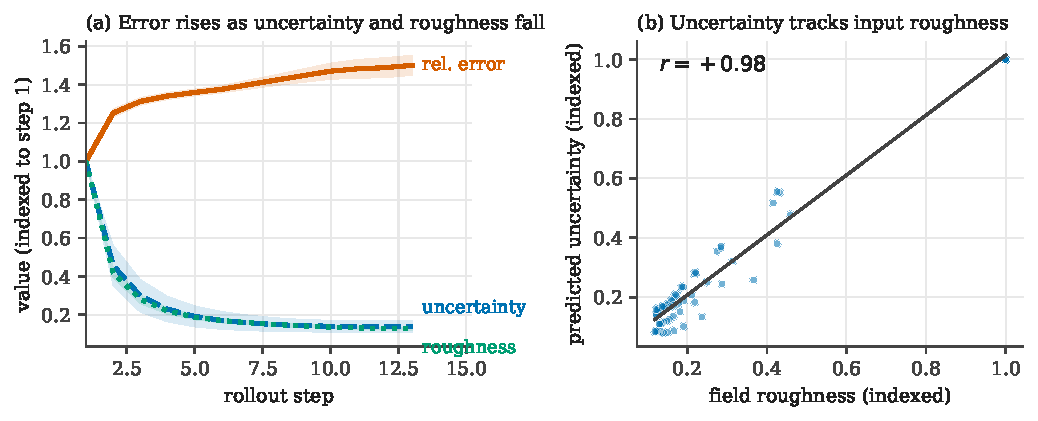
\includegraphics[width=\columnwidth]{img/rollout_drift.pdf}
    \caption{Mechanism of the rollout failure, averaged over the six schemes.
    (a) Indexed to the first rollout step, the relative error rises while the predicted
    uncertainty and the field roughness ($\overline{|\nabla \omega|}$) collapse together to
    $\sim\!13\%$. (b) Pooled over all schemes and steps, predicted uncertainty is an almost
    deterministic increasing function of the input field's roughness ($r = 0.98$). The model's
    uncertainty tracks how rough the current input looks, not how wrong the prediction is.}
    \label{fig:rollout}
\end{figure}

\textbf{Key findings}: (1) The result is the mirror image of Experiment 5 and is uniform across
schemes: as rollout error grows by $\sim\!1.5\times$, predicted uncertainty \emph{collapses} to
$8$--$17\%$ of its initial value, anti-correlated with error at a mean step correlation of $-0.94$.
(2) The model becomes more confident precisely as it drifts further from the true dynamics---the
same over-confidence-under-shift failure observed for parameter extrapolation in
Experiment~4. (3) The mechanism unifies Experiments 5 and 6: the predicted uncertainty is a
pointwise, learned function of the \emph{current input's local structure}, calibrated only
in-distribution. Sharp inputs (shocks) are read as uncertain and are indeed hard, so uncertainty
tracks error; but the FNO's spectral smoothing drives the autoregressive state toward blurred,
low-gradient fields that the model reads as easy---smooth yet increasingly wrong---so uncertainty
falls exactly when it should rise. Fig.~\ref{fig:rollout} makes this quantitative: across all six
schemes the predicted uncertainty tracks the field roughness $\overline{|\nabla \omega|}$ at a mean
correlation of $0.99$ (while roughness itself falls to $\sim\!13\%$ and anti-correlates with error),
so the reported uncertainty is effectively a readout of input smoothness rather than of prediction
error. (4) As in Experiment~5, the failure is cross-family, not evidential-specific: MC Dropout and
Deep Ensemble both collapse under rollout (uncertainty growth $0.17\times$ and $0.09\times$; step
correlation $-0.918$ and $-0.905$) and their uncertainty tracks input roughness just as tightly
(corr $0.985$ and $0.984$). The sampling-based methods estimate uncertainty from prediction
\emph{disagreement}, yet they too grow confident as the rollout state smooths, because every member
reads the same blurred input as easy. Faithful uncertainty under distribution shift therefore requires
a mechanism sensitive to global departure from the training manifold, not the pointwise evidence
used here (Sec.~\ref{sec:limitations})---and this requirement is shared by the sampling-based
baselines, not unique to evidential learning.

\subsection{Experiment 7: Architectural Ablation}

We ablate key components from the Log-Barrier evidential FNO using 3500 sample as train set and 1500 sample for test set. The Baseline row refers to the full Log-Barrier model with all default components intact, serving as the reference for comparison.

\begin{table}[htbp]
\centering
\caption{Ablation study. NaN indicates model failure (constant predictions).}
\label{tab:ablation}
\resizebox{\columnwidth}{!}{%
\begin{tabular}{lcccc}
\toprule
\textbf{Variant} & \textbf{MSE} $\downarrow$ & \textbf{rel\_l2} $\downarrow$ & \textbf{Calib.} $\downarrow$ & \textbf{Corr.} $\uparrow$ \\
\midrule
Baseline & \textbf{0.00194} & 0.0442 & 0.029 & 0.455 \\
\midrule
no\_skip\_connections & 0.996 & 1.000 & 0.339 & NaN \\
fourier\_only & 0.996 & 1.000 & 0.374 & NaN \\
no\_activations & 0.040 & 0.201 & 0.105 & 0.416 \\
with\_batch\_norm & 0.004 & 0.066 & 0.038 & 0.420 \\
\midrule
shallow\_heads & 0.002 & 0.045 & 0.029 & 0.447 \\
linear\_heads & 0.003 & 0.057 & 0.037 & 0.457 \\
with\_residual & 0.002 & \textbf{0.043} & \textbf{0.028} & 0.452 \\
\bottomrule
\end{tabular}%
}
\end{table}

\textbf{Key findings}: (1) Skip connections are critical---removing causes catastrophic failure (MSE $\approx$ 1.0). (2) Pure Fourier convolution without local components also fails completely. (3) Activations are necessary---removal causes 20$\times$ MSE degradation. (4) Batch normalization harms performance (2.2$\times$ worse). (5) Evidential head complexity matters little---shallow or linear heads maintain similar performance with fewer parameters. (6) Global residual connections provide modest improvement ($\sim$5\%).

\textbf{Design recommendations}: Required---skip connections, GELU activations. Recommended---global residuals. Optional---shallow evidential heads. Avoid---batch normalization.

\begin{figure*}[htbp]
    \centering
    \begin{subfigure}[b]{0.48\textwidth}
        \includegraphics[width=\textwidth]{img/exp6_ablation_performance.png}
        \caption{Prediction accuracy (MSE, rel$L^2$)}
    \end{subfigure}
    \hfill
    \begin{subfigure}[b]{0.48\textwidth}
        \includegraphics[width=\textwidth]{img/exp6_ablation_calibration.png}
        \caption{Calibration metrics}
    \end{subfigure}
    \caption{Architectural ablation results. Removing skip connections or using pure Fourier convolution causes catastrophic failure (MSE$\approx$1.0). Batch normalization degrades performance 2.2$\times$. Evidential head complexity (shallow vs. linear) has minimal impact on final performance.}
    \label{fig:exp6_ablation}
\end{figure*}  % Experiments
\section{Discussion}

\subsection{Evidential Methods for Neural Operators}

Our experiments establish evidential deep learning as the preferred approach for uncertainty quantification in 
neural operators. Key advantages include:

\textbf{Superior calibration}: Evidential methods (ECE $\sim$ 0.004) outperform MC Dropout (0.019) and Deep 
Ensembles (0.011) while maintaining 93--95\% coverage. This superiority holds across both Navier-Stokes and 
Darcy Flow, with the performance gap widening on harder problems.

\textbf{Computational efficiency}: Single-pass inference provides 5--30$\times$ speedup over alternatives, 
critical for real-time applications and high-throughput scientific computing workflows.

\textbf{Informative uncertainty}: Uncertainty-error correlation of 0.61 (vs. 0.31--0.33 for baselines) indicates 
evidential uncertainty better reflects prediction quality.

\textbf{MC Dropout unsuitable}: Across all metrics, MC Dropout exhibits inferior performance 
(6$\times$ worse MSE, lowest correlation), confirming it should be avoided for neural operators. 
The spatial coherence of PDE solutions may be incompatible with dropout's stochastic regularization.

\subsection{The Calibration-Decomposition Trade-off}

A fundamental limitation emerges from our decomposition analysis: methods achieving tight calibration 
(ECE $\sim$ 0.004) exhibit invalid decomposition (aleatoric variation $>$ 89\%), while valid decomposition 
(KL-Divergence) yields poor calibration (ECE = 0.030).

This trade-off appears intrinsic to the NIG parameterization. During training, the network increases evidence ($\nu, \alpha$) for correct predictions, directly reducing epistemic uncertainty ($\propto 1/\nu$). However, aleatoric uncertainty ($= \beta/(\alpha-1)$) also decreases because the loss function optimizes $\beta$ to match observed prediction variance. As the model improves with more data, prediction errors decrease, so the optimal $\beta$ decreases. Since $\alpha$ increases while $\beta$ decreases, the ratio $\beta/(\alpha-1)$ drops substantially---even though it theoretically should remain constant as irreducible data noise. The NIG parameterization lacks separate constraints to preserve aleatoric stability.

\textbf{Practical implication}: Practitioners should treat evidential outputs as \emph{total uncertainty} 
rather than interpreting the decomposition. For applications requiring true epistemic-aleatoric separation, 
Deep Ensembles remain preferable despite computational cost.

\subsection{Reinterpreting OOD Detection}

The stark contrast between parameter-level OOD (AUROC = 0.55) and operator-level OOD (AUROC = 1.0) suggests a 
domain-specific interpretation: parameter extrapolation within the same PDE family may not constitute true 
distributional shift from the operator learning perspective.

The FNO learns the Navier-Stokes operator in Fourier space, which generalizes across Reynolds numbers despite 
different flow characteristics. This explains maintained confidence at Re = 5000. Conversely, cross-PDE transfer 
represents genuine operator-level shift where the governing equations differ fundamentally, yielding appropriate 
massive uncertainty increases (36--378$\times$).

This finding has deployment implications: evidential uncertainty reliably monitors operator-level distributional 
shift but should not be solely relied upon for parameter extrapolation validation.

\subsection{Architectural Insights}

Our ablation study identifies critical components for evidential FNOs:
\begin{itemize}
    \item \textbf{Essential}: Skip connections and GELU activations---removal causes catastrophic failure
    \item \textbf{Beneficial}: Global residual connections (+5\% improvement)
    \item \textbf{Detrimental}: Batch normalization (2.2$\times$ worse), likely interfering with NIG parameter 
    learning
    \item \textbf{Flexible}: Evidential head complexity matters little---shallow heads maintain quality with fewer 
    parameters
\end{itemize}

\subsection{Limitations}

This study has several limitations: (1) evaluation on two PDEs (Navier-Stokes, Darcy Flow) may not generalize to 
other PDE families; (2) single architecture (FNO) tested---other operators may behave differently; (3) 
synthetic training data may not capture real-world measurement noise; (4) limited OOD scenarios tested. 
Future work should validate findings across broader PDE classes, architectures, and real-world applications.

\section{Conclusion}

This paper presents comprehensive comparison of uncertainty quantification methods for Fourier Neural Operators,
 evaluating MC Dropout, Deep Ensembles, and Evidential Deep Learning across calibration, efficiency, 
 decomposition validity, and OOD detection.

\textbf{Key findings}:
\begin{enumerate}
    \item Evidential methods achieve state-of-the-art calibration (ECE = 0.004) with single-pass inference, 
    outperforming MC Dropout (5$\times$ better ECE) and Deep Ensembles (3$\times$ better ECE) while being 
    5--30$\times$ faster.

    \item Uncertainty decomposition fails for well-calibrated evidential methods---both epistemic and aleatoric 
    uncertainties decrease with training data, revealing a fundamental calibration-decomposition trade-off in 
    the NIG parameterization.

    \item OOD detection capability depends critically on shift type: near-random for parameter extrapolation 
    (AUROC = 0.55) but perfect for operator-level shift (AUROC = 1.0), suggesting neural operators learn 
    physics-informed representations.

    \item MC Dropout should be avoided for neural operators due to consistently poor performance across all metrics.
\end{enumerate}

\textbf{Recommendations}: For production deployment, use evidential FNO with Uncertainty-Aware or Improved 
regularization. Report total uncertainty only (ignore decomposition). Implement threshold-based fallback for 
operator-level OOD detection. Reserve Deep Ensembles for applications requiring robust epistemic uncertainty despite 
computational cost.

Future work should investigate alternative parameterizations overcoming the calibration-decomposition trade-off, 
extend evaluation to broader PDE families and architectures, and develop physics-informed OOD metrics for parameter 
extrapolation scenarios.  % Discussion and Conclusion

% ==================== ACKNOWLEDGMENT ====================
\section*{Acknowledgment}
The authors would like to express their sincere gratitude to National Taiwan University of Science and Technology for 
their valuable support in conducting this research. Their collaboration, academic resources, and institutional 
encouragement have been instrumental in the successful completion of this study.

The authors used Anthropic Claude language polishing (grammar, readability, and style). These tools were not 
used to generate data, conduct analyses, or produce the study's results. The authors reviewed and approved all 
revisions and assume full responsibility for the submitted work.

% ==================== REFERENCES ====================
\bibliographystyle{IEEEtran}
\bibliography{references}

% ==================== APPENDIX ====================
\clearpage
\onecolumn
\appendices

\section{Notation Reference}
\label{app:notation}

%Table~\ref{tab:notation} summarizes the mathematical symbols used throughout this paper.

\begin{table}[!ht]
\centering
\caption{Summary of mathematical notation.}
\label{tab:notation}
\begin{tabular}{lll}
\toprule
\textbf{Symbol} & \textbf{Description} & \textbf{Section} \\
\midrule
\multicolumn{3}{l}{\textit{PDE and Neural Operator}} \\
$a(x)$ & Input function (e.g., initial condition, permeability field) & Prelim. \\
$u(x)$ & Output/solution function & Prelim. \\
$\mathcal{G}_\theta$ & Neural operator parameterized by $\theta$ & Prelim. \\
$\mathcal{L}$ & PDE operator & Prelim. \\
$\omega$ & Vorticity (Navier-Stokes) & Experiments \\
$\nu_{\text{visc}}$ & Viscosity coefficient & Experiments \\
$k(x)$ & Permeability field (Darcy flow) & Experiments \\
\midrule
\multicolumn{3}{l}{\textit{FNO Architecture}} \\
$\mathcal{F}, \mathcal{F}^{-1}$ & Fourier transform and inverse Fourier transform & Prelim. \\
$\mathcal{K}$ & Spectral convolution operator & Prelim. \\
$\mathbf{w}, R$ & Learnable weights in Fourier space & Prelim. \\
$v_l(x)$ & Latent representation at Fourier layer $l$ & Prelim. \\
$W_l$ & Skip connection (local linear) weights at layer $l$ & Prelim. \\
$P$ & Lifting layer (input $\rightarrow$ latent space) & Prelim. \\
$Q, Q^{\text{evid}}$ & Projection layer (vanilla / evidential) & Method. \\
$\sigma(\cdot)$ & Activation function (GELU) & Prelim. \\
$L$ & Number of Fourier layers & Prelim. \\
$w$ & FNO width (latent channel dimension) & Method. \\
$H, W$ & Spatial grid dimensions & Method. \\
$d_{in}$ & Number of input channels & Method. \\
\midrule
\multicolumn{3}{l}{\textit{Uncertainty Quantification Methods}} \\
$T$ & Number of MC Dropout forward passes & Prelim. \\
$M$ & Number of ensemble members & Prelim. \\
$p$ & Dropout rate & Method. \\
$\mu$ & Predictive mean & Prelim. \\
$\sigma^2$ & Predictive variance & Prelim. \\
$\hat{y}_t$ & Prediction at MC Dropout pass $t$ & Prelim. \\
$\hat{y}_m$ & Prediction of ensemble member $m$ & Prelim. \\
\midrule
\multicolumn{3}{l}{\textit{Normal-Inverse-Gamma (NIG) Distribution}} \\
$\gamma$ & Predicted mean (location parameter) & Prelim. \\
$\nu$ & Evidence parameter (precision of mean estimate) & Prelim. \\
$\alpha$ & Shape parameter ($> 1$) & Prelim. \\
$\beta$ & Scale parameter ($> 0$) & Prelim. \\
$\sigma^2_{\text{ale}}$ & Aleatoric uncertainty $= \beta / (\alpha - 1)$ & Prelim. \\
$\sigma^2_{\text{epi}}$ & Epistemic uncertainty $= \beta / [\nu(\alpha - 1)]$ & Prelim. \\
$\Omega$ & NIG loss auxiliary term $= 2\beta(1 + \nu)$ & Method. \\
$\Gamma(\cdot)$ & Gamma function & Prelim. \\
$\psi(\cdot)$ & Digamma function & Method. \\
\midrule
\multicolumn{3}{l}{\textit{Training and Regularization}} \\
$\mathcal{L}_{\text{NIG}}$ & NIG negative log-likelihood loss & Method. \\
$\mathcal{L}_{\text{reg}}$ & Regularization loss term & Method. \\
$\lambda$ & Regularization strength & Method. \\
$\lambda_\nu$ & Evidence regularization strength (Improved, L2) & Method. \\
$\lambda_{\text{KL}}$ & KL divergence regularization strength & Method. \\
$D_{\text{KL}}$ & KL divergence & Method. \\
$\eta$ & Learning rate & Experiments \\
$\epsilon$ & Numerical stability constant ($10^{-6}$) & Method. \\
\midrule
\multicolumn{3}{l}{\textit{Evaluation Metrics}} \\
$N$ & Number of test samples & Prelim. \\
$y_i, \hat{y}_i$ & Ground truth and predicted values & Prelim. \\
$\hat{\sigma}_i$ & Predicted uncertainty for sample $i$ & Prelim. \\
$\rho$ & Uncertainty-error Pearson correlation & Prelim. \\
$z_\alpha$ & Confidence level critical value & Prelim. \\
\bottomrule
\end{tabular}
\end{table}

% ==================== BIOGRAPHIES ====================
\twocolumn
\vfill

\begin{IEEEbiography}[{
\includegraphics[width=1in,height=1.25in,clip,keepaspectratio]{img/self-photo.jpeg}}]{Ahmad Rifqi}
received the B.S. degree in computer engineering from Universitas Indonesia, Depok, Indonesia, in 2025. He is 
currently pursuing the M.S. degree with the Department of Electrical and Computer Engineering, 
National Taiwan University of Science and Technology (NTUST), Taipei, Taiwan. His research interests include 
deep learning, uncertainty quantification, and scientific machine learning.
\end{IEEEbiography}

\begin{IEEEbiography}[{
\includegraphics[width=1in,height=1.25in,clip,keepaspectratio]{img/profleu.jpeg}}]{Jenq-Shiou Leu}
(Senior Member, IEEE) received the B.S. degree in mathematics and the M.S. degree in computer science and 
information engineering from National Taiwan University, Taipei, Taiwan, in 1991 and 1993, respectively, and 
the Ph.D. degree on a part-time basis in computer science from National Tsing Hua University, Hsinchu, Taiwan, 
in 2006. He was with Rising Star Technology, Taiwan, as an R\&D Engineer from 1995 to 1997, and was with 
telecommunication industry (Mobitai Communications and Taiwan Mobile) from 1997 to 2007 as an Assistant Manager. 
In 2007, he joined the Department of Electronic and Computer Engineering, National Taiwan University of Science 
and Technology, Taiwan, as an Assistant Professor. From 2011 to 2014, he was an Associate Professor. Since 2014, 
he has been a Professor. His research interests include heterogeneous network integration, mobile service and 
platform design, distributed computing (P2P, cloud computing), green and orange technology integration. He has 
authored or coauthored extensively in these areas, with 114 SCI-indexed papers and 76 conference papers.
\end{IEEEbiography}

\end{document}